% Copyright 2021 Politecnico di Milano, Italy. Inc. All rights reserved

\documentclass{PoliMi_MasterThesis}

% === Packages and configurations ===
% Configurations
\usepackage{parskip} % For paragraph layout
\usepackage{setspace} % For using single or double spacing
\usepackage{emptypage} % To insert empty pages
\setlength\parindent{0pt} % Indentation
\raggedbottom % Do not stretch empty space to fill the page

% Titles
\usepackage{titlesec}
% \titlespacing{\section}{left spacing}{before spacing}{after spacing}
\titlespacing{\section}{0pt}{3.3ex}{2ex}
\titlespacing{\subsection}{0pt}{3.3ex}{1.65ex}
\titlespacing{\subsubsection}{0pt}{3.3ex}{1ex}
\usepackage{color}

% Language and fonts
\usepackage[english]{babel} % The document is in English  
\usepackage[utf8]{inputenc} % UTF8 encoding
\usepackage[T1]{fontenc} % Font encoding
\usepackage[11pt]{moresize} % Big fonts

% Images
\usepackage{graphicx} % For images
\graphicspath{{./Images/}} % Directory of the images
\usepackage{transparent} % Enables transparent images
\usepackage{eso-pic} % For the background picture on the title page
\usepackage{subfig} % Numbered and caption subfigures using \subfloat.
\usepackage{tikz} % A package for high-quality hand-made figures.
\usetikzlibrary{}
\usepackage{caption} % Coloured captions
\usepackage{xcolor} % Coloured captions
\usepackage{amsthm,thmtools,xcolor} % Coloured "Theorem"
\usepackage{float}
\usepackage[font=small]{caption} % To make captions small
\usepackage{eso-pic} % Background pictures for each page
\newcommand*\triangleLogo{
	\clearpage
	\thispagestyle{empty}
	\newpage
	\begin{figure}
		\centering
		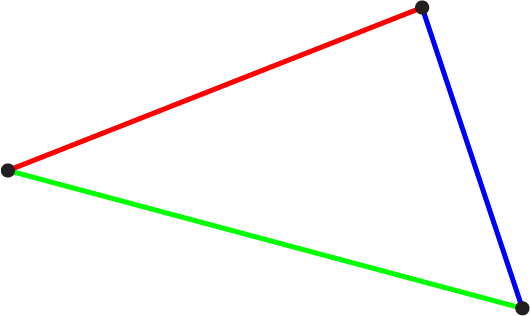
\includegraphics[width=\textwidth]{Images/triangle_logo_thin.png} 
	\end{figure}
}

% Math
\usepackage{amsmath}
\usepackage{amsthm}
\usepackage{amssymb}
\usepackage{amsfonts}
\usepackage{bm}
\usepackage[overload]{empheq} % For braced-style systems of equations.
\usepackage{fix-cm} % To override original LaTeX restrictions on sizes

% Tables
\usepackage{tabularx}
\usepackage{longtable} % Tables that can span several pages
\usepackage{colortbl}

% Algorithms
\usepackage{algorithm}
\usepackage{algorithmicx}
\usepackage{algpseudocodex}
\newcommand*\Let[2]{\State #1 $\gets$ #2}
\newcommand*\AAnd{\textbf{ and }}
\newcommand*\AOr{\textbf{ or }}

% Bibliography
\usepackage[colorlinks=true,linkcolor=black,anchorcolor=black,citecolor=black,filecolor=black,menucolor=black,runcolor=black,urlcolor=black]{hyperref} % Adds clickable links at references
\usepackage{cleveref}
\usepackage[square, numbers, sort&compress]{natbib} % Square brackets, citing references with numbers, citations sorted by appearance in the text and compressed
\bibliographystyle{abbrvnat} % You may use a different style adapted to your field

% Other packages
\usepackage{pdfpages} % To include a pdf file
\usepackage{afterpage}
\usepackage{fancyhdr} % For the headers
\fancyhf{}

% Input of configuration file. Do not change config.tex file unless you really know what you are doing. 
% Set the geometric layout of the document
\usepackage{geometry}
\geometry{
  top=3cm,
  left = 1.5cm,
  right = 1.5cm,
  bottom=2cm,
  headheight= 2cm,
  headsep= 0cm,
}
\raggedbottom 

% Create color bluePoli (-> manuale grafica coordinata:  https://www.polimi.it/fileadmin/user_upload/il_Politecnico/grafica-coordinata/2015_05_11_46xy_manuale_grafica_coordinata.pdf)
\definecolor{bluePoli}{cmyk}{0.4,0.1,0,0.4}

% Custom theorem environments
\declaretheoremstyle[
  headfont=\color{bluePoli}\normalfont\bfseries,
  bodyfont=\color{black}\normalfont\itshape,
]{colored}

\captionsetup[figure]{labelfont={color=bluePoli}} % Set colour of the captions
\captionsetup[table]{labelfont={color=bluePoli}} % Set colour of the captions
\captionsetup[algorithm]{labelfont={color=bluePoli}} % Set colour of the captions

\theoremstyle{colored}
\newtheorem{theorem}{Theorem}[section]
\newtheorem{proposition}{Proposition}[section]

% Enhances the features of the standard "table" and "tabular" environments.
\newcommand\T{\rule{0pt}{2.6ex}}
\newcommand\B{\rule[-1.2ex]{0pt}{0pt}}

% Algorithm description
\newcounter{algsubstate}
\renewcommand{\thealgsubstate}{\alph{algsubstate}}
\newenvironment{algsubstates}{
    \setcounter{algsubstate}{0}%
    \renewcommand{\STATE}{%
    \stepcounter{algsubstate}%
    \Statex {\small\thealgsubstate:}\space}
    }{}
    
% Custom theorem environment
\newcolumntype{L}[1]{>{\raggedright\let\newline\\\arraybackslash\hspace{0pt}}m{#1}}
\newcolumntype{C}[1]{>{\centering\let\newline\\\arraybackslash\hspace{0pt}}m{#1}}
\newcolumntype{R}[1]{>{\raggedleft\let\newline\\\arraybackslash\hspace{0pt}}m{#1}}

% Custom itemize environment
\setlist[itemize,1]{label=$\bullet$}
\setlist[itemize,2]{label=$\circ$}
\setlist[itemize,3]{label=$-$}
\setlist{nosep}

% Set separation of columns 
\setlength{\columnsep}{30pt}

% Create command for background pic
\newcommand\BackgroundPic{% Adding background picture
	\put(198,330){
		\parbox[b][\paperheight]{\paperwidth}{%
			\vfill
			\centering
			\transparent{0.4}
			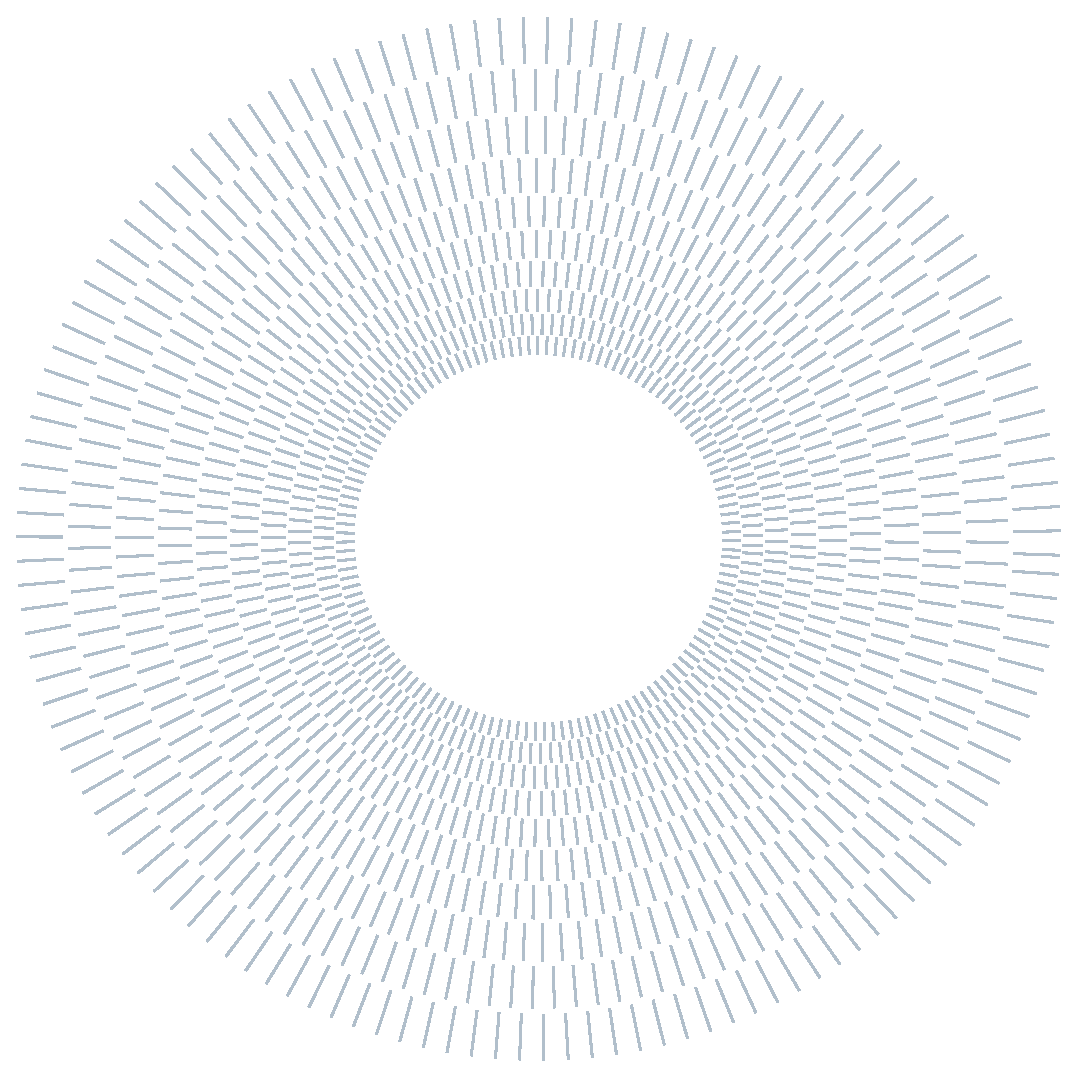
\includegraphics[width=0.7\paperwidth]{raggiera_polimi.eps}%
			\vfill
}}}

% Set indentation
\setlength\parindent{0pt}

% Custom title commands
\titleformat{\section}
{\color{bluePoli}\normalfont\Large\bfseries}
{\color{bluePoli}\thesection.}{1em}{}
\titlespacing*{\section}
{0pt}{2ex}{1ex}

\titleformat{\subsection}
{\color{bluePoli}\normalfont\large\bfseries}
{\color{bluePoli}\thesubsection.}{1em}{}
\titlespacing*{\subsection}
{0pt}{2ex}{1ex}

% Custom headers and footers
\pagestyle{fancy}
\fancyhf{}
      
\fancyfoot{}
\fancyfoot[C]{\thepage} % page
\renewcommand{\headrulewidth}{0mm} % headrule width
\renewcommand{\footrulewidth}{0mm} % footrule width

\makeatletter
\patchcmd{\headrule}{\hrule}{\color{black}\hrule}{}{} % headrule
\patchcmd{\footrule}{\hrule}{\color{black}\hrule}{}{} % footrule
\makeatother

% -> Create the header
\chead[C]{
\centering
\begin{tcolorbox}[arc=0pt, boxrule=0pt, colback=bluePoli!60, width=\textwidth, colupper=white]
    \textsc{\textbf{Executive summary}} \hfill \textsc{\textbf{\author}} 
\end{tcolorbox}
}


% === Start of document ===

\begin{document}
\fancypagestyle{plain}{
\fancyhf{} % Clear all header and footer fields
\fancyhead[R]{\thepage} %RO=right odd, RE=right even
\renewcommand{\headrulewidth}{0pt}
\renewcommand{\footrulewidth}{0pt}}


% === Title page ===
\pagestyle{empty} % No page numbers
\frontmatter % Use roman page numbering style (i, ii, iii, iv...) for the preamble pages

\puttitle{
	title=Ray Distribution Aware Heuristics for Bounding Volume Hierarchies Construction,
	name=Lapo Falcone,
	course=Computer Science and Engineering,
	ID  = 996089,
	advisor= Prof. Marco Gribaudo,
	academicyear={2023-24}
}


% === Preamble ===
\startpreamble
\triangleLogo
\setcounter{page}{1} % Set page counter to 1

% Abstract
\makeatletter
\let\savedchap\@makechapterhead
\def\@makechapterhead{\vspace*{-3cm}\savedchap}
\polimichapter{Abstract}
\let\@makechapterhead\savedchap
\makeatletter
\small
In the last few years, real-time computer graphics have been transitioning from a pipeline based on rasterization to one using ray tracing.
Ray tracing makes it possible to accurately simulate the behavior of light rays, enabling developers of graphics content to reproduce high-fidelity scenes without using a plethora of techniques to mimic light transport.

While ray tracing is widely used for off-line rendering, such as for CGI effects in films or animated movies, the same cannot be stated for on-line applications, such as videogames. The main problem with ray tracing is that simulating light transport is computationally expensive, reason why in recent videogames ray tracing is only used on small portions of the scene or to simulate some effects (such as reflections, shadows, or ambient occlusion).

In order to increase the spread of ray tracing in on-line rendering applications too, research is moving in two macro directions.

The first one is to build GPUs with an architecture more suited for ray tracing, such as the RT cores from Ampere Nvidia GPUs.

The second, but not least important one is to design software optimizations to make ray tracing cheaper.

One of the problems that is ubiquitous in the ray tracing environment is to detect collisions between a ray and the geometry of the scene to render. Given the huge amount of primitives present in modern graphic applications, it is necessary to use a data structure to accelerate the ray collision retrieval process. The state-of-the-art structure is the bounding volume hierarchy (BVH), which hierarchically organizes primitives, making it possible to skip entire sections of the scene that are spatially far away from the ray that is being traced during BVH traversal.

In this work we propose two novel heuristics that work in pairs to build higher-quality BVHs, a data structure to make it possible to use them, and a comparative analysis of their performance in different scenarios.

The first heuristic, called \textbf{projected area heuristic} (PAH), aims at better estimating the amount of rays that hit each node of the BVH by exploiting some artifacts in the ray distribution in the scene, caused by another optimization used in a previous step of the ray tracing pipeline (namely Monte-Carlo importance sampling).

The second one (\textbf{splitting plane facing}) aims at reducing the overlap among nodes of the BVH, consequently reducing the number of intersection tests needed during the BVH traversal phase.

\textbf{Keywords:} Ray tracing, bounding volume hierarchy, BVH
\normalsize

% Abstract in Italian
\makeatletter
\let\savedchap\@makechapterhead
\def\@makechapterhead{\vspace*{-3cm}\savedchap}
\polimichapter{Abstract in Lingua Italiana}
\let\@makechapterhead\savedchap
\makeatletter
\small
Abstract Italiano
\\
\\
\textbf{Parole chiave:} Ray tracing, bounding volume hierarchy, BVH
\normalsize


% === Table of contents ===
\thispagestyle{empty}
\tableofcontents % Table of contents 
\thispagestyle{empty}
\cleardoublepage

\addtocontents{toc}{\vspace{2em}} % Add a gap in the Contents, for aesthetics
\mainmatter % Begin numeric (1,2,3...) page numbering

% Add logo to page numbers
\AddToShipoutPicture{%
	\put(\textwidth+58,\textheight+88){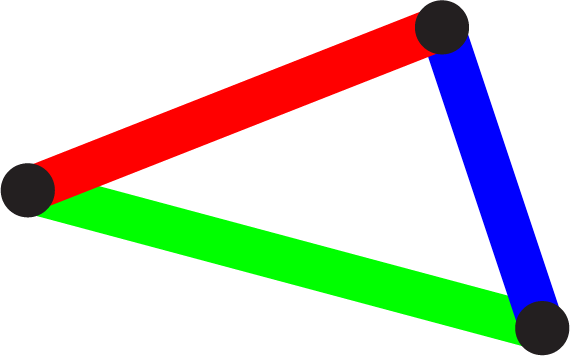
\includegraphics[scale=0.06]{Images/triangle_logo.png}}
}

% === Intro ===
\chapter*{Introduction}
\large \textbf{Why ray tracing?} \normalsize\\
In the field of computer graphics, we refer to ray tracing as a family of rendering algorithms that simulate light transport in order to transition from a mathematical representation of a scene to an image on the screen. 

TODO same in chapter 1
Conceptually ray tracing is an extremely straightforward technique, that can be summarized in a few steps:
\begin{enumerate}
\item Generate a ray of light from a light source;
\item Find out the first object the ray intersects;
\item Compute how much energy is absorbed by the material of the object;
\item Modify the direction of the ray based on the material of the object (for example it may be reflected or refracted);
\item Repeat from 2. until the ray hits the camera;
\item Color the pixel of the camera hit by the ray based on the energy of the ray.
\end{enumerate}

\begin{figure}[H]
    \centering
    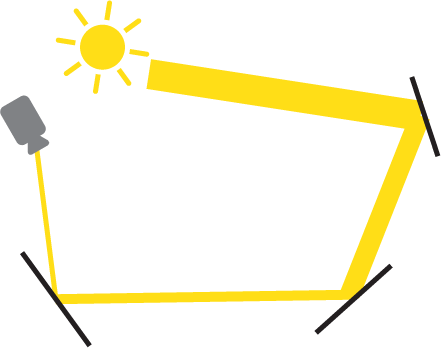
\includegraphics[scale=0.4]{Images/ray_tracing_simple.png}
    \caption{The width of the yellow ray represents the amount of energy carried. After each intersection some energy is absorbed.}
    \label{fig:ray_tracing_simple}
\end{figure}

Since ray tracing mimics the behavior of light in the real world, the technique can be directly used to simulate complex light effects that would require the use of ad-hoc and approximate methods if we use other rendering algorithms, such as the widely spread rasterization pipeline.

To give an intuition of how the ad-hoc methods can be convoluted and produce worse results, we summarize one of the most intuitive ones used to generate shadows, called shadow mapping. A shadow map is the projection of the scene from the point of view of a point light source, saved in a texture where each pixel stores the distance from the light source to the projected point. When the scene is projected by the main camera, each visible point is transformed into the coordinate system of the shadow map via matrix multiplication, and is then compared to the point stored in the corresponding pixel of the shadow map. If the point of the shadow map is closer to the light source than the corresponding point projected by the main camera, we deduce that such a point is not visible from the point of view of the light source and, therefore, is in shadow. This specific technique is correct only with point lights, and must be adjusted in case translucent objects are present in the scene.

With ray tracing shadows are natively generated since, if a point is in shadow, no light ray starting from it will hit the camera pixels. Moreover, in principle, it works with any kind of light, not only point lights, and thus produces higher-quality shadows, since no approximations must be made.

\large \textbf{We need optimizations} \normalsize\\
Until now we briefly highlighted the strong points of ray tracing, and greatly simplified it. The main issue with ray tracing is that it is computationally expensive to simulate light transport. Of course, it is impossible to track the path of every photon emitted by a light source, therefore, even in ray tracing algorithms, some approximations must be made. The nature of the approximations depends on the specific ray tracing algorithm used. For example, in many techniques falling under the name of \textit{backward ray tracing} \footnote{In some literature the term \textit{backward ray tracing} can also refer to the opposite family of algorithms, since the first ray tracing methods were indeed backward.}, rays don't start from the light sources, but from the camera, and gain energy when they hit a light source. At this point the path described by the ray is followed backward and the energy hitting the pixel of the camera is computed. In this way the number of rays is greatly reduced, because all the rays hit the camera, therefore none is wasted. On the other hand, some phenomena (such as caustics) cannot be realistically simulated.

From this point on we will consider the scenario where rays are traced backwards.

One optimization that is foundational to modern ray tracing and relevant to our work, is the use of the \textbf{Monte-Carlo} integration method, and, in particular, a variance reduction technique called \textbf{importance sampling}. We will introduce the concept in this section in an oversimplified way, and then explain it from a mathematical standpoint in \ref{TODO}.

When a ray hits a point on a surface, it may bounce in any direction, based on the material. The most intuitive bounce is a perfect reflection, but, since at a microscopic level surfaces are never perfectly planar, it is possible for the incoming ray to bounce in any direction. This phenomenon is described in a probabilistic way by the bidirectional reflective distribution function (BRDF). Each material is described by a BRDF, and each BRDF makes it more likely for a ray coming from a certain direction to bounce to another range of directions (for example, for a perfectly reflective material, the BRDF will return a probability of 1 for a ray to bounce to the perfect reflection direction).

\begin{figure}[H]
    \centering
    \subfloat[Perfectly reflective surface.]{
        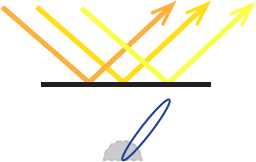
\includegraphics[scale=0.45]{Images/reflective_brdf.png}
		}
		\qquad
	\subfloat[Non-reflective surface.]{
        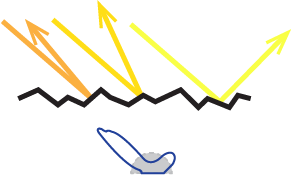
\includegraphics[scale=0.45]{Images/non_reflective_brdf.png}
    }
	\caption{In figure (a) all the rays coming from a direction are reflected towards the same direction. In (b), instead, the surface is microscopically rough, 2 rays coming from the same direction could bounce to 2 very different directions. Under each figure there is the corresponding graph of its BRDF.} 
    \label{fig:surfaces_reflectiveness}
\end{figure}

Therefore, if we wanted to accurately simulate the light behavior after a ray hits a material, and compute how much light is reflected towards a specific direction (the one of the incoming ray), we would need to send a probe ray to every direction of the hemisphere centered on the hit point, get back the light energy carried by each probe ray, and compute an average based on the probability of each probe ray given by the BRDF. In short, we would need to integrate the light energy function over the hemisphere. This exact same process would then need to be replicated when each probe ray hits an object, recursively, until each ray in the scene hits a light source or gets completely absorbed.

This process, of course, is not feasible, but it can be approximated by the Monte-Carlo method with fewer samples. The idea is that, instead of probing each direction of the hemisphere with a ray, we probe just a small number (often just one) of directions. In most cases the estimate of the light incoming to the point will not be accurate, but, granted that there is a high enough number of incoming rays hitting the neighborhood of the point, the incoming light average will indeed be accurate.

In order to get the most out of the probe rays we cast out of a hemisphere, we would like to send them in directions that contribute the most to the final value we are trying to calculate, namely the light reflected toward the direction of the incoming ray. This is the base concept behind importance sampling. In ray tracing there are two common ways to achieve this:
\begin{description}
\item[BRDF sampling] Probe rays are cast in directions where the BRDF returns a high weight. In this way the energy the probe rays carry is multiplied by a value close to 1; on the other hand, the energy can be a low value.
\item[Light sampling] Probe rays are cast directly towards light sources. In this way they will likely carry a lot of energy (unless an obstacle is hit), but the BRDF weight they will be multiplied with may be small.
\end{description}
It is even possible to combine the two techniques with a method called multiple importance sampling (MIS).

The use of importance sampling generates artifacts in the ray distribution on the scene. Rays' directions will no longer be distributed uniformly, but, due to light sampling, more rays will tend to go towards light sources.

\large \textbf{Rays intersections} \normalsize\\
One of the problems that is common to all the algorithms of the ray tracing family is to find the intersection between a ray and the geometry of the scene.

The objects in the scene are usually meshes, which are a collection of geometric primitives. In many real-world scenarios, primitives are simple triangles, described by 3 vertices. Therefore, the problem of intersecting a ray with the scene is reduced to the problem of intersecting a ray with a collection of triangles.

Given an algorithm to find out if a ray hits a triangle in \ref{sec:ray_triangle_intersection}, the naive way of retrieving the closer triangle hit by a ray would be to perform the ray-triangle test on all the triangles present in the scene. Such an algorithm has a complexity of $\mathcal{O}(n\cdot m)$ where $n$ is the number of triangles and $m$ the number of rays.

Acceleration structures have been developed to speed up the process. The state-of-the-art acceleration structure used in ray tracing is the \textbf{bounding volume hierarchy} (BVH).

In summary, a BVH is a binary tree\footnote{Technically it can be a tree with any breadth, but binary trees are the most common ones.} where each node wraps some of the triangles in the scene in a bounding volume, usually an axis-aligned bounding box (AABB). Given a node $A$ wrapping the triangles in the set $T_A$, the two children of $A$, called $B$ and $C$ wrap the triangles in the sets $T_B$ and $T_C$ such that $T_B \cup T_C = T_A$. Thanks to this structure, if a ray doesn't intersect a bounding volume, we deduce that it will not intersect any of the triangles contained in the bounding volume too, making it possible to discard them without having to perform any additional intersection test. This means that, if the BVH is balanced, the the complexity to find an intersection between a ray and the scene is $\mathcal{O}(log_2(n) \cdot m)$.

\begin{figure}[H]
    \centering
    
\includegraphics[scale=0.4]{Images/TODO.png}
    \caption{A 2-dimensional BVH.}
    \label{fig:bvh_2d}
\end{figure}

Given the definition and the advantages of a BVH over the naive algorithm, we now have to build a BVH starting from the primitives in the scene.
Building the optimal BVH is an NP-complete problem since, for each level of the BVH, we would have to try all the possible ways to subdivide the triangles into 2 AABBs, recursively, until all the branches are leaves; then measure the quality of the BVHs and take the best one.

In a real-world scenario a greedy algorithm is used instead, where, at each level, some of the possible ways to subdivide the triangles are tried, and the best one with reference to a cost metric function is greedily taken. This means that, even if in the next level it is found out that the split in a previous level was not optimal, the algorithm proceeds without changing the previous decision.

The quality of the trees built with such an algorithm depends on many factors, but two of the most relevant ones are the cost function and how the algorithm tries to split the triangles at each level.

\large \textbf{The surface area heuristic} \normalsize\\
The vast majority of the state-of-the-art algorithms to build BVHs uses the \textbf{surface area heuristic (SAH)} as cost metric. SAH is extremely simple and fast: the cost of a node $K$ is proportional to the probability that a random ray intersects the node $p(hit\:K)$, and the number of primitives the node contains $\#T_K$:
$$SAH(K) = p(hit\:K) \cdot \#T_K$$

The probability that a node is hit by a random ray is proportional to its area: $p(hit\:K) = \frac{A_K}{A_tot}$ where $A_tot$ is the area of the AABB enclosing the whole scene.
Computing the area of an AABB is trivial.

SAH is based on three hypotheses:
\begin{enumerate}
	\item All the rays hit AABB enclosing the whole scene.
	\item All the rays start from outside the scene.
	\item Rays are distributed in a uniform random way on their 6-dimensional space (3 dimensions for the position of their origin and 3 dimensions for their direction).
\end{enumerate}

None of these hypotheses is satisfied in a real-world scenario, and, in particular, we will focus on the third one.

As we noted above, due to the use of importance sampling, rays are not distributed uniformly in the scene. In particular, due to light sampling, in proximity of light sources, rays have directions pointing towards the light source. Based on the light source type, we have different types of ray distributions, as it is possible to appreciate in the images below.

\begin{figure}[H]
    \centering
    \subfloat[Point light generated distribution]{
        
\includegraphics[scale=0.25]{Images/TODO.png}
		}
		\qquad
	\subfloat[Area light generated distribution]{
        
\includegraphics[scale=0.25]{Images/TODO.png}
    }
	\caption{The ray distributions generated by point and area lights.}
    \label{fig:generated_distributions}
\end{figure}

Area lights tend to generate regions where rays are parallel. This means that we can better estimate the probability that a ray intersects an AABB by computing its projected area on the plane perpendicular to the bundle of rays, instead of the surface area of the AABB. Such a projected area can be computed with an orthographic projection.

Point lights, instead, tend to generate a bundle of lines passing through a point, and therefore the projected area can be computed with a perspective projection.

In this work we aim to show how this way of computing the cost function for the construction of a BVH can produce higher quality BVHs in some situations. We named this novel approach as \textbf{projected area heuristic (PAH)}.





% === Chapter 1 ===
\chapter{Background Theory}
\label{ch:background_theory}
In this chapter we will summarize the background knowledge needed to fully comprehend this work.

In section \ref{sec:ray_tracing_principles} we will introduce ray tracing in simple terms, and list some of its advantages, disadvantages and its today's applications.

In section \ref{sec:monte_carlo_and_variance_reduction_techniques} we will analyze from a mathematical standpoint how the most used ray tracing algorithms work.

Last, in section \ref{sec:ray_tracing_acceleration_structures}, we will describe the state-of-the-art acceleration structure to make a fundamental ray tracing procedure (ray-scene intersection) faster.

\section{Ray Tracing Principles} \label{sec:ray_tracing_principles}
\subsection*{High Level Overview}
Ray tracing is a family of rendering algorithms that is used in computer graphics to transition from a mathematical representation of a scene, to an image on the screen.

Conceptually ray tracing is an extremely straightforward technique, that can be summarized in a few steps:
\begin{enumerate}
\item Generate a ray of light from a light source;
\item Find out the first object the ray intersects;
\item Compute how much energy is absorbed by the material of the object;
\item Modify the direction of the ray based on the material of the object (for example it may be reflected or refracted);
\item Repeat from 2. until the ray hits the camera or loses all its energy;
\item Color the pixel of the camera hit by the ray based on the energy of the ray.
\end{enumerate}

Ray tracing aims to mimic the real-world behavior of light, and for this reason it can be directly employed to simulate any light effect, starting from the simplest ones, such as perfect reflections and shadows, going towards the most complex ones, such as global illumination and caustics. Some of the most accurate ray tracing algorithms can even simulate quantum effects of light \cite{quantum_ray_tracing}.

Since ray tracing natively simulates light, it can produce extremely realistic images, without resorting to ad-hoc techniques used to approximate light phenomena in other rendering algorithms, such as the widely spread rasterization pipeline.

To give an intuition of how the ad-hoc methods can be convoluted and produce worse results, we summarize one of the simplest ones used to generate shadows, called shadow mapping \cite{shadow_maps}. A shadow map is the projection of the scene from the point of view of a point light source, saved in a texture where each pixel stores the distance from the light source to the projected point. When the scene is projected by the main camera, each visible point is transformed into the coordinate system of the shadow map via matrix multiplication (figure \ref{fig:shadow_map}). The point in the new coordinate system is then compared to the point stored in the corresponding pixel of the shadow map. If the point of the shadow map is closer to the light source than the corresponding point projected by the main camera, we deduce that such a point is not visible from the point of view of the light source and, therefore, is in shadow. This specific technique is correct only with point lights, and must be adjusted in case translucent objects are present in the scene.

With ray tracing shadows are natively generated since, if a point is in shadow, no light ray starting from it will hit the camera pixels. Moreover, in principle, it works with any kind of light, not only point lights, and thus produces higher-quality shadows, since no approximations must be made.

\begin{figure}[]
    \centering
    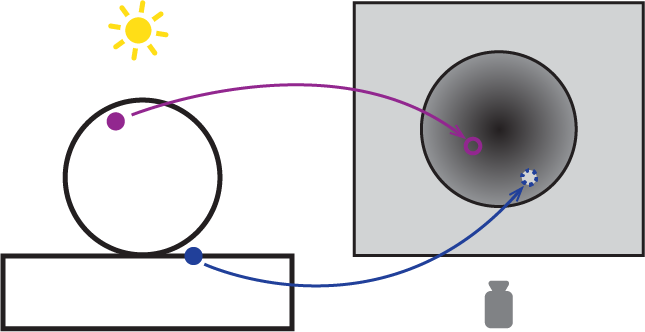
\includegraphics[scale=0.6]{Images/shadow_map.png}
    \caption{The first figure is from the main camera PoV, the second one from the light source PoV. The second figure represents depth: the closer a point is to the light source, the darker. The blue point is in shadow, because the corresponding point in the shadow map is further away than the stored depth.}
    \label{fig:shadow_map}
\end{figure}

\subsection*{Use Cases}
Due to the highly realistic images ray tracing algorithms can produce, the technique has found a lot of success in many applications. We can subdivide the use cases into two macro-categories: real-time ray tracing and production ray tracing.

The most prominent use of the second category is in movies. CGI effects and animated films are almost always produced by using ray tracing, in particular a very accurate algorithm called path tracing. In the first category we can find videogames.

The main difference between real-time and production ray tracing lies in the time constraints for producing a frame. In production ray tracing producing a frame can take a long time, even in the order of magnitude of days. Whereas, in real-time ray tracing, a frame must be produced every $33$ms to achieve $30$ frames per second (fps), and every $16.5$ms to achieve $60$ fps, which can be considered today's standard by many PC videogames.

This starking difference makes it so that different techniques must be used depending on the scenario. In real-time ray tracing many approximations must be introduced in order to stay within the frame time budget, whereas in production ray tracing more accurate algorithms can be used, since time constraints are loose. Our work can benefit both categories, since the methods we will introduce can make ray tracing faster, in some situations, without introducing approximations.

\subsection*{Optimizations Overview}
Until now we briefly highlighted the strong points of ray tracing, and greatly simplified it. The main issue with ray tracing is that it is computationally expensive to simulate light transport in a convincing way. The reason lies in the rendering equation, and will be explained in section \ref{sec:monte_carlo_and_variance_reduction_techniques}.

In order to make ray tracing usable in the real world, the industry moved in two directions:
\begin{description}
	\item [Hardware accelerators] GPU vendors, in particular Nvidia, started creating GPUs with specialized cores for ray tracing. These cores have a memory layout that makes it faster to find a ray-triangle intersection. An example of this can be the RT cores from Turing Nvidia GPUs \cite{rt_cores}.
	\item [Software optimizations] Software developers introduced new algorithms to improve the performance of a specific part of the ray tracing pipeline. These algorithms can vary a lot in complexity and results. One of the most common optimizations for real-time ray tracing is to use ray tracing only for some light effects (such as shadows or reflections), while using rasterization for most of the scene.
\end{description}

Software optimizations can, in turn, be subdivided into two big families.

Some optimizations aim at improving the time needed to detect the first intersection of a ray with the scene. These optimizations don't alter the quality of the rendered scene. We will diffusely talk about these optimizations in section \ref{sec:ray_tracing_acceleration_structures}, and this work can be placed into this family.

The other family comprehends optimizations aimed at reducing the number of rays needed to produce a visually acceptable image. This work, while being part of the first family of optimizations, has its foundations in an artifact in the ray distribution in the scene caused by an optimization in this second family. This technique is called importance sampling, and will be discussed in section \ref{sec:monte_carlo_and_variance_reduction_techniques}.

\subsection*{Backward Ray Tracing}
Before going to the next section, it is important to introduce the concept of backward ray tracing\footnote{In some literature the term \textit{backward ray tracing} can also refer to the opposite family of algorithms, since the first ray tracing methods were indeed backward.}. 

In backward ray tracing light rays don't start from light sources, but from the eye position. Starting from the eye, each ray will then hit a fictitious plane placed in front of the eye (the near plane), similar to what happens in a pinhole camera \ref{pinhole_camera}. The near plane can be subdivided into discrete units displaced in a regular grid, which we will consider the pixels of the final image. Each ray is therefore associated with the pixel it hits, and will contribute to its final color.

\begin{figure}[H]
    \centering
    
\includegraphics[scale=0.4]{Images/TODO.png}
    \caption{How rays are cast in backward ray tracing.}
    \label{fig:pinhole_camera}
\end{figure}

The rays starting from the camera will hit the scene and bounce around. At each bounce a ray loses a fraction of its energy (unless the surface is perfectly reflective), until either it gets completely absorbed, or it hits a light source. In the case a ray hits a light source, we already know how much of its energy will be lost due to intersections with objects, therefore we can immediately compute the color of the pixel associated with the ray (as if we followed that same ray's path backward). If a ray never hits a light source, it will not contribute to the color of its associated pixel.

A way of looking at this algorithm is to think we are tracing \textit{importons}, which can be considered the dual concept of \textit{photons} \cite{importons}. Thanks to the light reciprocity principle \cite{light_reciprocity}, which states that light transmits in the same way in both ways, tracing photons or importons is equivalent.

The advantage of backward ray tracing is that, with a limited budget of rays we can cast, it is more efficient than forward ray tracing. Indeed, in forward ray tracing it is possible a ray never hits the camera, in which case it would be wasted. In backward ray tracing all the rays hit the camera by definition, thus none is wasted.

Of course, if a ray starting from the camera never hits a light source, it could be considered wasted, but some techniques that will be described in section \ref{sec:monte_carlo_and_variance_reduction_techniques} makes it more likely that a ray hits a light source in its path.

From this point on we will consider the scenario where rays are traced backwards.

\section{Monte-Carlo and Variance Reduction Techniques} \label{sec:monte_carlo_and_variance_reduction_techniques}
In this section we will analyze the mathematical foundations of ray tracing, namely the Kajiya's rendering equation. Then we will present a statistical method to resolve the integrals appearing in the rendering equation, called Monte-Carlo. Finally, we will discuss a variance reduction technique, importance sampling, that can be used to obtain better approximations from the Monte-Carlo method. We will see how this technique generates artifacts in the ray distribution in the scene, which is one of the hypotheses of our thesis.

\subsection*{Kajiya's Rendering Equation}
$$
L_o(\bar{x},\bar{\omega}_o) = L_e(\bar{x}, \bar{\omega}_o) + \int_\Omega BRDF(\bar{x}, \bar{\omega}_i, \bar{\omega}_o) \cdot \cos(\bar{n}, \bar{\omega}_i) \cdot L_i(\bar{x}, \bar{\omega}_i) d\bar{\omega}_i
$$

This equation, developed by James T. Kajiya in 1986 \cite{rendering_equation}, can be used to calculate the amount of light \textit{generated} by a point $\bar{x}$ towards a direction $\bar{\omega}_o$. In order to compute such a quantity we need to know these parameters:
\begin{itemize}
	\item $L_e(\bar{x}, \bar{\omega}_o)$ The light emitted by the point $\bar{x}$ towards a direction $\bar{\omega}_o$.
	\item $BRDF$ The bidirectional reflectance distribution function of the material at point $\bar{x}$.
	\item $\bar{n}$ The normal to the surface at point $\bar{x}$.
	\item $L_i(\bar{x}, \bar{\omega}_i)$ The light incoming to $\bar{x}$ from a generic direction $\bar{\omega}_i$.
\end{itemize}

The equation can be divided into two parts:

The first part describes the light emitted $L_e(\bar{x}, \bar{\omega}_o)$, and it is 0 unless the point is a light source. Depending on the light source, it can assume a uniform value in each direction (point light), a value only in one hemisphere (a plane area light), or a specific value based on the direction, usually controlled by a function (such as in spotlight). In any case the emitted light value is known by the definition of the light source in the scene, therefore can be easily plugged into the equation.

The second part of the equation presents an integral, and represents the light reflected by the material of the point towards the direction $\bar{\omega}_o$. In simple words, this second term tells us that, in order to compute the reflected light, we have to know, first, how much light is incoming to the point from all the directions in the hemisphere $\Omega$. And second, the properties of the material, summarized in the $BRDF$. The $BRDF$ tells us how much of the incoming light is reflected towards the direction $\bar{\omega}_o$. 

\begin{figure}[H]
    \centering
    
\includegraphics[scale=0.3]{Images/TODO.png}
    \caption{A visual representation of the integral term of the rendering equation.}
    \label{fig:rendering_equation}
\end{figure}

The term $\cos(\bar{n}, \bar{\omega}_i)$ is called geometry term, and reflects a core property of light, independent of the $BRDF$. Indeed, based on the angle a beam of light intersects a surface, the beam of light will enlighten a smaller or bigger area of the surface. The smallest surface is illuminated when the direction of the beam of light and the normal to the surface are parallel. Since the energy carried by the beam of light is constant, we can deduce that, the bigger the enlightened surface, the lower the energy per area unit. In particular, if we let $L$ be the energy of the beam and $\alpha$ the angle between the beam direction and the normal, then the energy received per area unit equals to $L\cdot \cos(\alpha)$.

\begin{figure}[H]
    \centering
    
\includegraphics[scale=0.3]{Images/TODO.png}
    \caption{The geometry term.}
    \label{fig:geometry_term}
\end{figure}

In this integral term, the BRDF is known by definition, and the geometry term is a simple cosine. TODO instead the $L_i$ term can only be known by probing rays, and it is recursive ($L_in$ point 1 = $L_out$ point 2). Moreover, there is an integral, therefore Monte Carlo

\subsection*{Monte-Carlo}
\subsection*{Variance Reduction Techniques}

\section{Ray Tracing Acceleration Structures} \label{sec:ray_tracing_acceleration_structures}


% === Chapter 2 ... ===
\chapter{Chapter two}
Chapter 2


% === Bibliography ===
\addtocontents{toc}{\vspace{2em}} % Add a gap in the Contents, for aesthetics
\bibliography{Bibliography} % The references information are stored in the file named "Bibliography.bib"


% === Appendices ===
\cleardoublepage
\addtocontents{toc}{\vspace{2em}} % Add a gap in the Contents, for aesthetics
\appendix

\chapter{Collision and Culling Algorithms}
\section{Ray-AABB Intersection} \label{sec:ray_box_intersection}
The algorithm we used to detect intersections between a ray and an AABB is the branchless slab algorithm \cite{ray_box_intersection}.

Given a ray in the form: $r(t) = O + t\cdot d$, where $O$ is the origin and $d$ the direction, the main idea of the algorithm is to find the 2 values of $t$ ($\overline{t_1}$ and $\overline{t_2}$) such that $r(\overline{t_{1,2}})$ are the points where the ray intersects the AABB.

Since the object to intersect the ray with is an axis-aligned bounding box in the min-max form, the algorithm can proceed one dimension at a time:
\begin{enumerate}
	\item First, it finds the intersection points of the ray with the planes parallel to the $yz$ plane, and sorts them in an ascending order with reference to the corresponding $\overline{t_{1,2}}$ values. We call the point with the smallest $\overline{t}$ value the \textit{closest}, and the other one the $\overline{furthest}$.
	\item Then it does the same with the $xz$ plane:
	\begin{itemize}
		\item As closest intersection point, it keeps the furthest between the 2 closest intersection points found so far (the one with the $yz$ plane and the one with the $xz$ plane).
		\item As furthest intersection point, it keeps the closest between the 2 furthest intersection points found so far.
	\end{itemize}
	\item Then it does the same with the $xy$ plane.
	\item Finally, an intersection is detected only in the case where the furthest intersection point actually has an associated $\overline{t}$ value bigger than the one of the closest point found by the algorithm.
	\item The returned $\overline{t}$ value is the smaller one, as long as it is greater or equal to 0; otherwise it means that the origin of the ray is inside the AABB, and one of the intersection points is \textit{behind} the ray origin.
\end{enumerate}
	
\begin{figure}[H]
    \centering
    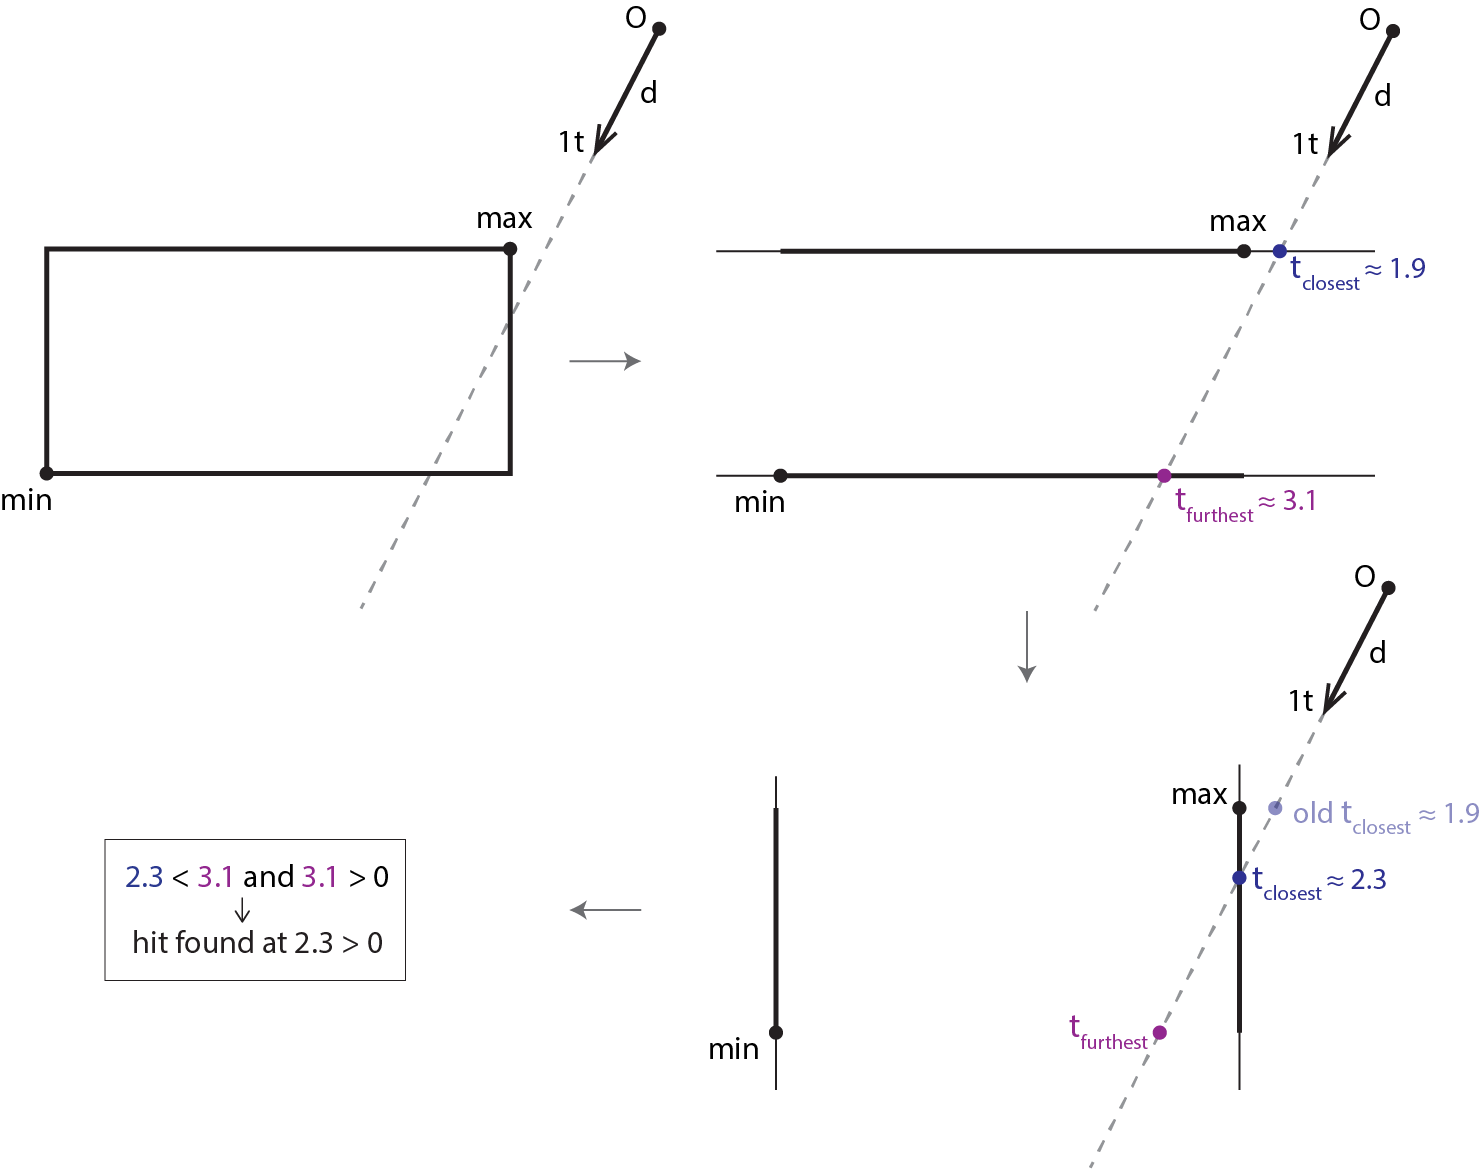
\includegraphics[width=\textwidth]{Images/ray_aabb_intersection.png}
    \caption{Visual representation of the presented algorithm in 2 dimensions. An interactive simulation of this algorithm can be found at: \url{https://www.geogebra.org/m/np3tnjvb}.}
    \label{fig:ray_aabb_intersection}
\end{figure}

\begin{algorithm}[H]
	\caption{Ray-AABB branchless slab intersection algorithm in 3 dimensions}
	\begin{algorithmic}[1]
		\Function{Intersect}{$ray, aabb$}
		\Let {$t1_x$}{$\frac{aabb.min.x - ray.origin.x}{ray.direction.x}$} \Comment{yz plane}
		\Let {$t2_x$}{$\frac{aabb.max.x - ray.origin.x}{ray.direction.x}$}
		\Let {$tMin$}{$min(t1_x, t2_x)$}
		\Let {$tMax$}{$max(t1_x, t2_x)$}
		\Let {$t1_y$}{$\frac{aabb.min.y - ray.origin.y}{ray.direction.y}$} \Comment{xz plane}
		\Let {$t2_y$}{$\frac{aabb.max.y - ray.origin.y}{ray.direction.y}$}
		\Let {$tMin$}{$ max(tMin, min(t1_y, t2_y))$}
		\Let {$tMax$}{$ min(tMax, max(t1_y, t2_y))$}
		\Let {$t1_z$}{$\frac{aabb.min.z - ray.origin.z}{ray.direction.z}$} \Comment{xy plane}
		\Let {$t2_z$}{$\frac{aabb.max.z - ray.origin.z}{ray.direction.z}$}
		\Let {$tMin$}{$max(tMin, min(t1_z, t2_z))$}
		\Let {$tMax$}{$min(tMax, max(t1_z, t2_z))$}
		\Let {$areColliding$}{$tMax > tMin$ \AAnd $tMax \geq 0$}
		\Let {$collisionDist$}{$tMin < 0 \: ? \: tMax \: : \: tMin$}
		\State \Return $\langle areColliding, collisionDist \rangle$
		\EndFunction
	\end{algorithmic}
\end{algorithm} 

It is interesting to note how, under the floating-point IEEE 754 standard, the algorithm also works when it is not possible to find an intersection point along a certain axis (i.e. when the ray is parallel to certain planes). Indeed, in such cases, the values $\overline{t_{1,2}}$ will be $\pm \infty$, and the comparisons will still be well defined.

\section{Ray-Plane Intersection} \label{sec:ray_plane_intersection}
For ray-plane intersection we decided to use this algorithm presented in the educational portal of the SIGGRAPH conference \cite{ray_plane_intersection}.

Given a ray in the form: $r(t) = O + t\cdot d$, where $O$ is the origin and $d$ the direction, and a plane whose normal $n$ and a point $P$ are known, we first check whether the plane and the ray are parallel, in which case no intersection can be found.

Then, if they are not parallel, we obtain the analytic form of the 3-dimensional plane: 
\begin{align*}
	A\cdot x + B\cdot y + C\cdot z + D = 0
\end{align*}
In particular, we know a point $P$ that is part of the plane, therefore we can obtain the $D$ parameter:
\begin{align*}
&A\cdot P_x + B\cdot P_y + C\cdot P_z + D = 0\\
\implies& D = -(A\cdot P_x + B\cdot P_y + C\cdot P_z)
\end{align*}
By definition, the vector formed by the parameters $[A,B,C]$ is perpendicular to the plane, therefore:
\begin{align*}
&D = -(n_x\cdot P_x + n_y\cdot P_y + n_z\cdot P_z)\\
\implies& D = -\langle n \cdot P \rangle
\end{align*}
Now that we have the parametric equation of the plane, we can force a point of the plane to also be a point of the ray: 
\begin{align*}
	&A\cdot r(t)_x + B\cdot r(t)_y + C\cdot r(t)_z + D = 0\\
	\implies& A\cdot (O_x + t\cdot d_x) + B\cdot (O_y + t\cdot d_y) + C\cdot (O_z + t\cdot d_z) + D = 0\\
	\implies& t = \frac{-\langle n\cdot O \rangle + D}{\langle n\cdot d \rangle}
\end{align*}
Finally, if the found $\overline{t}$ value is negative, it means that the intersection point between the ray and the plane is \textit{behind} the ray origin, therefore no intersection is found. Else the ray intersects the plane at point $r(\overline{t})$.

\begin{algorithm}[H]
	\caption{Ray-plane intersection algorithm}
	\begin{algorithmic}[1]
		\Function{Intersect}{$ray, plane$}
		\Let{$d$}{$ray.direction$}
		\Let{$O$}{$ray.origin$}
		\Let{$n$}{$plane.normal$}
		\Let{$P$}{$plane.point$}
		\If{$\langle n\cdot d \rangle = 0$} \Comment{Ray is parallel to plane}
			\State \Return $\langle false, \_ \rangle$
		\EndIf
		\Let{$D$}{$-\langle n\cdot P \rangle$}
		\Let{$t$}{$\frac{-\langle n\cdot O \rangle}{\langle n\cdot d \rangle}$}
		\If{$t<0$} \Comment{Intersection point is \textit{behind} ray origin}
			\State \Return $\langle false, \_ \rangle$
		\Else
			\State \Return $\langle true, t \rangle$
		\EndIf
		\EndFunction
	\end{algorithmic}
\end{algorithm} 

\section{Ray-Triangle Intersection} \label{sec:ray_triangle_intersection}
Once we have algorithms to check for ray-plane intersection (\ref{sec:ray_plane_intersection}) and for a point inside a 2D convex hull (\ref{sec:point_inside_2dHull}), we can combine them to check if a ray intersects a triangle and to compute the coordinates of the intersection point:

\begin{enumerate}
	\item Build a plane that has as normal the normal to the triangle, and as point any vertex of the triangle;
	\item Use the ray-plane intersection algorithm (\ref{sec:ray_plane_intersection}) to find the coordinates of the point where the ray and the plane collide (if any);
	\item Use the point inside 2D convex hull test (\ref{sec:point_inside_2dHull}) to determine if the intersection point is inside the triangle.
\end{enumerate}

\section{AABB-AABB Intersection} \label{sec:aabb_aabb_intersection}
To detect a collision between 2 axis-aligned bounding boxes in the min-max form, it is sufficient to check that there is an overlap between them in all 3 dimensions. By naming the 2 AABBs as $A$ and $B$ we get:
\begin{subequations}
	\begin{align*}[left=\empheqlbrace]
		A.min_x \leq& B.max_x \\
		A.max_x \geq& B.min_x \\
		A.min_y \leq& B.max_y \\
		A.max_y \geq& B.min_y \\
		A.min_z \leq& B.max_z \\
		A.max_z \geq& B.min_z
	\end{align*}
\end{subequations}

\section{Frustum-AABB Intersection} \label{sec:frustum_aabb_intersection}
In order to detect an intersection between a frustum and an axis-aligned bounding box in the min-max form, we used a simplified version of the separating axis test (a special case of the separating hyperplane theorem) \cite{separating_axis_test}. The simplification comes from the fact that we need to find the intersection of a frustum and an AABB, and not two 3D convex hulls, meaning that we can exploit some assumptions on the direction of the edges of the two objects, as we'll note below.

Before proceeding with the separating axis test, we first try a simpler AABB-AABB collision test, between the given AABB and the AABB that most tightly encloses the frustum. In case this \textit{rejection test} gives a negative answer, we can deduce that the frustum and the AABB are not colliding. Otherwise, we must use the more expensive SAT.

The separating axis theorem in 3 dimensions states that 2 convex hulls are not colliding if and only if there is a plane that divides the space into 2 half-spaces each fully containing one of the two convex hulls.\\
To find whether such a plane exists, we project the two convex hulls on certain axes, and check whether their 1D projections are overlapping. The theorem also states that if there is an axis where the projections are not overlapping it must be either:
\begin{itemize}
	\item An axis perpendicular to one of the faces of the convex hulls, or
	\item An axis parallel to the cross product between an edge of the first convex hull and an edge of the second convex hull.
\end{itemize}
This consideration makes it possible to use the theorem in a concrete scenario.

\begin{figure}[H]
    \centering
    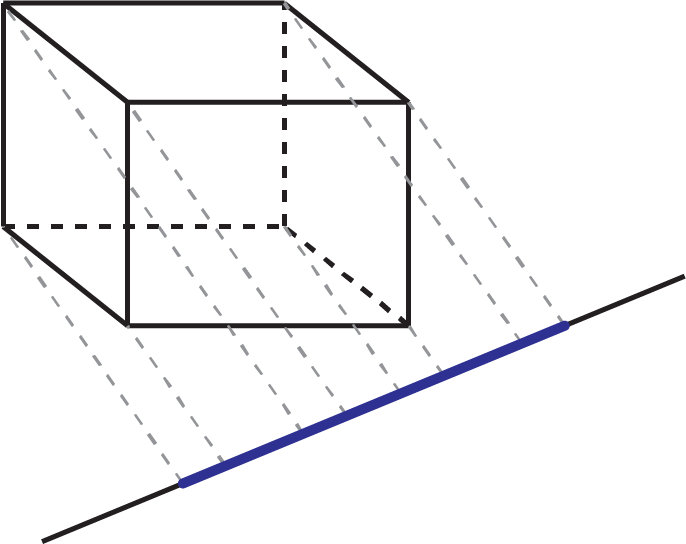
\includegraphics[scale=0.35]{Images/aabb_1d_proj.png} 
    \caption{The projection of an AABB on an axis.}
    \label{fig:aabb_1d_proj}
\end{figure}

In principle, given 2 polyhedra with 6 faces each (such as a frustum and an AABB), there should be $(6 + 6)_{normals} + (12\cdot 12)_{cross\: products} = 156$ axis to check; but, since:
\begin{itemize}
	\item The AABB has edges only in 3 different directions, and faces normals only in 3 different directions, and
	\item The frustum has edges only in 6 different directions, and faces normals only in 5 different directions
\end{itemize}
the number of checks is reduced to $(3 + 5)_{normals} + (3\cdot 6)_{cross\: products} = 26$.

\begin{figure}[H]
    \centering
    \subfloat[AABB: 3 different edges directions]{
        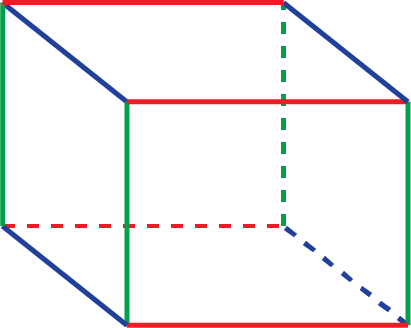
\includegraphics[scale=0.35]{Images/aabb_edges_same_dir.png}
		}
		\qquad
	\subfloat[Frustum: 6 different edges directions]{
        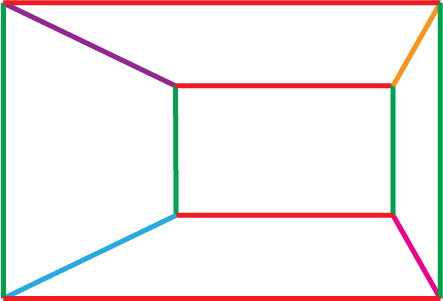
\includegraphics[scale=0.35]{Images/frustum_edges_same_dir.png}
    }
	\caption{In the figure the edges having the same direction are colored in the same color.}
    \label{fig:aabb_frustum_different_edges_directions}
\end{figure}


\subsection{1D Projections Overlapping Test}
In order to detect if the 1D projections of the 3D hulls are overlapping, we identify the outermost points of each projection (namely $A_{min}, A_{max}, B_{min}, B_{max}$) and check that $B_{min} \leq A_{max} \And B_{max} \geq A_{min}$.\\
For the AABB another optimization is possible, where we detect what points will be the outermost after the projection without actually projecting them, based on the direction of the axis:

\begin{figure}[H]
    \centering
    \subfloat[AABB vertices layout.]{
        \raisebox{-0.1\height}{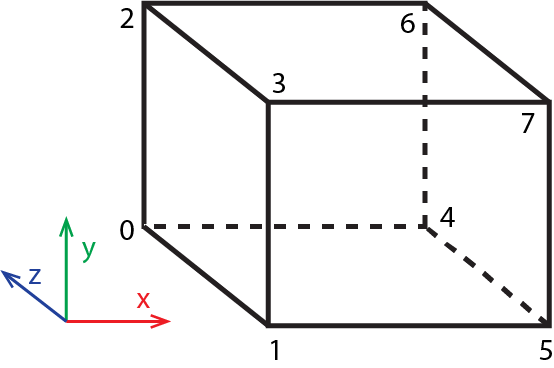
\includegraphics[scale=0.35]{Images/aabb.png}}
    }
    \quad
    \subfloat{
		\raisebox{0.5\height}{
		\begin{tabular}{| c | c |}
			\hline
			\textbf{axis direction} & \textbf{extremes} \\
			\hline \hline
			$x \geq 0 \And y \geq 0 \And z \leq 0$ & 1, 6\\
			$x \leq 0 \And y \leq 0 \And z \geq 0$ & 6, 1\\
			$x \geq 0 \And y \geq 0 \And z \geq 0$ & 0, 7\\
			$x \leq 0 \And y \leq 0 \And z \leq 0$ & 7, 0\\
			$x \geq 0 \And y \leq 0 \And z \leq 0$ & 3, 4\\
			$x \leq 0 \And y \geq 0 \And z \geq 0$ & 4, 3\\
			$x \geq 0 \And y \leq 0 \And z \geq 0$ & 2, 5\\
			$x \leq 0 \And y \geq 0 \And z \leq 0$ & 5, 2\\
			\hline
		\end{tabular}
		}
    }
    \label{fig:aabb_projected_extremes}
\end{figure}

\begin{algorithm}[H]
	\caption{Ray-AABB branchless slab intersection algorithm in 3 dimensions}
	\begin{algorithmic}[1]
		\Function{Intersect}{$frustum, aabb$}
		\If{$!intersect(frustum.aabb, aabb)$} \Comment{AABB-AABB test}
			\State \Return $false$
		\EndIf
		\Let{$axesToCheck$}{$(\perp frustum \: faces) \cup (\perp AABB \: faces) \cup (\times edges$)}
		\ForAll{$axis \in axesToCheck$}
			\Let{$frustumExtremes$}{$findFrustumExtremes(frustum, axis)$} \Comment{Returns the vertices of the frustum that, after the projection, will be the extremes}
			\Let{$aabbExtremes$}{$findAabbExtremes(aabb, axis)$} \Comment{Same as above, but uses the discussed optimization}
			\Let{$A_{min}$}{$\langle aabbExtremes.first \cdot axis \rangle$}
			\Let{$A_{max}$}{$\langle aabbExtremes.second \cdot axis \rangle$}
			\Let{$B_{min}$}{$\langle frustumExtremes.first \cdot axis \rangle$}
			\Let{$B_{max}$}{$\langle frustumExtremes.second \cdot axis \rangle$}
			\If{$!(B_{min} \leq A_{max} \And B_{max} \geq A_{min})$} 
				\State \Return $false$
			\EndIf
		\EndFor
		\State \Return $true$ \Comment{If we havent't found any axis where there is no overlap, boxes are colliding}
		\EndFunction
	\end{algorithmic}
\end{algorithm} 

\section{Point inside AABB Test} \label{sec:point_inside_aabb}
To check if a point $P$ is inside an axis-aligned bounding box in the min-max form, it is sufficient to compare its coordinates with the minimum and maximum of the AABB component-wise:
\begin{subequations}
	\begin{align*}[left=\empheqlbrace]
		min_x \leq P_x \leq max_x \\
		min_y \leq P_y \leq max_y \\
		min_z \leq P_z \leq max_z
	\end{align*}
\end{subequations}

\section{Point inside Frustum Test} \label{sec:point_inside_frustum}
It is possible to detect whether a point is inside a 3-dimensional frustum by projecting it with the perspective matrix associated with the frustum and then comparing its coordinates, as suggested by \cite{point_inside_frustum_test}.

Given the perspective matrix $\textit{M}$ associated with the frustum, we can project a point $P$ and get: $P' = \textit{M} \cdot P$; and perform the perspective division. 

$P'' = \frac{P'}{P'_w}$ $P''$ is now in normalized device coordinates (NDC) space, where the frustum is an axis-aligned bounding box that extends from $\langle -1, -1, -1 \rangle$ to $\langle 1, 1, 1 \rangle$ \footnote{Based on the convention used, it is possible that the AABB in NDC space has a different size. For example, it is common an AABB extending from $\langle -1, -1, 0 \rangle$ to $\langle 1, 1, 1 \rangle$}.

It is now immediate to see that $P$ is inside the frustum if and only if $P''$ is inside the AABB (see section \ref{sec:point_inside_aabb}).

A simple optimization allow us to avoid the perspective division. Indeed, since in homogeneous coordinates:
$$\langle x',y',z',w' \rangle = \langle \frac{x'}{w'},\frac{y'}{w'},\frac{z'}{w'},\frac{w'}{w'} \rangle = \langle x'',y'',z'',1 \rangle$$
We can change the inequalities to check whether the point is inside the frustum from:

\begin{minipage}{.4\linewidth}
	\begin{subequations}
		\begin{align*}[left=\empheqlbrace]
			-1 \leq x'' \leq 1 \\
			-1 \leq y'' \leq 1 \\
			-1 \leq z'' \leq 1
		\end{align*}
	\end{subequations}
\end{minipage}
		to:
\begin{minipage}{.4\linewidth}
	\begin{subequations}
		\begin{align*}[left=\empheqlbrace]
			-w' \leq x' \leq w' \\
			-w' \leq y' \leq w' \\
			-w' \leq z' \leq w'
		\end{align*}
	\end{subequations}
\end{minipage}

We created a 2D visual demonstration of how it is possible to detect if a point is inside a frustum at \url{https://www.geogebra.org/m/ammj5mxd}.

\section{Point inside 2D Convex Hull Test} \label{sec:point_inside_2dHull}
Given a 2D convex hull in 3-dimensional space and a 3D point laying on the same plane as the hull, it is possible to use a simple inside-outside test \cite{ray_triangle_intersection} to determine whether the point is inside the convex hull.

The main idea is that the point lays inside the convex hull if and only if it is \textit{to the right} (or \textit{to the left}, depending on the winding order) of all the edges of the hull.

In order to determine the relative position of a point and an edge $\overline{AB}$, we can look at the cross product:
$$u \times v \; where \; u = \overrightarrow{AB}, v = \overrightarrow{AP}$$

\begin{figure}[H]
    \centering
    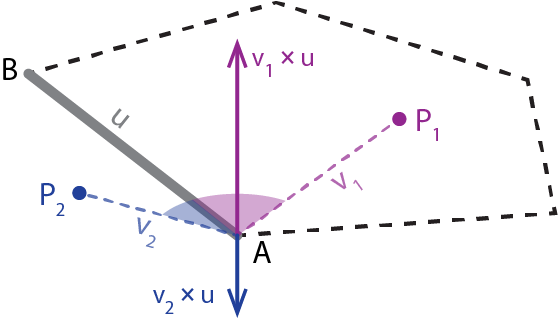
\includegraphics[scale=0.4]{Images/cross_product.png} 
    \caption{Visualization of cross product.}
    \label{fig:cross_product}
\end{figure}

Therefore the strategy to determine if a point is on the same side of all the edges of the convex hull is to compute a reference cross product, by choosing any of the edges, and then making sure that all the other cross products have the same direction. To check that 2 vectors have the same direction it is sufficient that their dot product is positive.

\begin{algorithm}[H]
	\caption{Inside-outside test between a 3D point and a 2D convex hull.} 
	\begin{algorithmic}[1]
		\Function{IsInside}{$P, hull$}
		\Let{$N$}{$number \: of \: edges \: of \: hull$}
		\Let{$u$}{$hull[0] - hull[N-1]$}
		\Let{$v$}{$P - hull[N-1]$}
		\Let{$ref$}{$u \times v$} \Comment{The reference cross product}
		\For{$0\leq i < N$}
			\Let{$u$}{$hull[i+1] - hull[i]$}
			\Let{$v$}{$P - hull[i]$}
			\Let{$cross$}{$u \times v$}
			\If{$\langle ref \cdot cross \rangle \leq 0$}
				\State \Return $false$
			\EndIf
		\EndFor
		\State \Return $true$
		\EndFunction
	\end{algorithmic}
\end{algorithm} 

\section{2D Convex Hull Culling} \label{sec:2dHull_culling}
In order to find the overlapping region between two 2D hulls in 2-dimensional space, we can proceed as illustrated in the diagram below (\cite{convex_hull_culling}):

\begin{figure}[H]
    \centering
    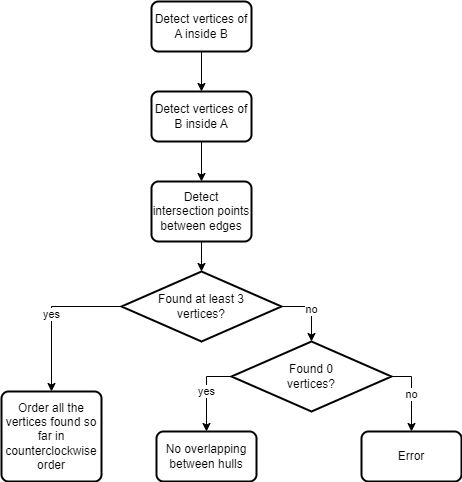
\includegraphics[scale=0.7]{Images/hull_culling.png} 
    \caption{General algorithm to find the overlapping region between two convex hulls called $A$ and $B$.}
    \label{fig:hull_culling}
\end{figure}

\begin{figure}[H]
    \centering
    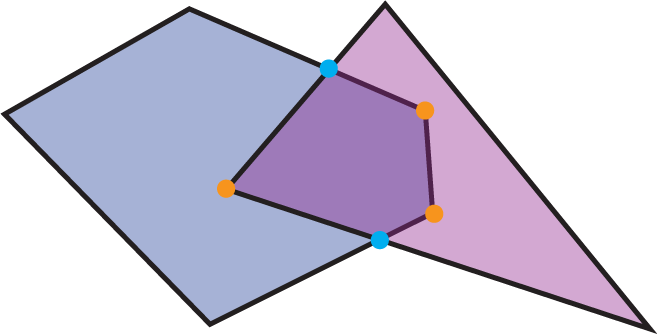
\includegraphics[scale=0.4]{Images/overlapping_hull.png} 
    \caption{Yellow vertices are found in the first 2 steps (vertices inside), whereas light blue vertices are found in the third step (edges intersections).}
    \label{fig:overlapping_hull}
\end{figure}

We'll now go through each phase and see the used algorithms.

\subsection{Vertices inside convex hull}
To find out what vertices of a hull are inside the other one we simply looped over them and used the point inside convex hull test (\ref{sec:point_inside_2dHull}).

\subsection{Edges intersections}
To detect an intersection between two segments, we first have to compute the equation of the line the segment is lying on.

Given a segment $\overline{PQ}$, the underlying line has equation:
$$A\cdot x + B\cdot y = C$$
We can then compute the parameters of the line as:
\begin{subequations}
	\begin{align*}[left=\empheqlbrace]
		A &= Q_y - P_y\\
		B &= P_x - Q_x\\
		C &= A\cdot P_x + B\cdot P_y
	\end{align*}
\end{subequations}

After we calculate the underlying line of both segments, with parameters $A_1, B_1, C_1, A_2, B_2, C_2$, we can compute the intersection point $K$ of the two lines as:
\begin{subequations}
	\begin{align*}[left=\empheqlbrace]
		\Delta &= A_1 \cdot B_2 - A_2 \cdot B_1\\
		K_x &= \frac{B_2 \cdot C_1 - B_1 \cdot C_2}{\Delta}\\
		K_y &= \frac{A_1 \cdot C_2 - A_2 \cdot C_1}{\Delta}
	\end{align*}
\end{subequations}

We are now left with the task of verifying whether the found intersection point $K$ is in between both segments' extremes. Let's call the first segment $\overline{MN}$ and the second one $\overline{PQ}$:

\begin{minipage}{.4\linewidth}
	\begin{subequations}
		\begin{align*}[left=\empheqlbrace]
			min(M_x, N_x) &\leq K_x \And\\
			max(M_x, N_x) &\geq K_x \And\\
			min(M_y, N_y) &\leq K_y \And\\
			max(M_y, N_y) &\geq K_y		
		\end{align*}
	\end{subequations}
\end{minipage}
		$And$
\begin{minipage}{.4\linewidth}
	\begin{subequations}
		\begin{align*}[left=\empheqlbrace]
			min(P_x, Q_x) &\leq K_x \And\\
			max(P_x, Q_x) &\geq K_x \And\\
			min(P_y, Q_y) &\leq K_y \And\\
			max(P_y, Q_y) &\geq K_y		
		\end{align*}
	\end{subequations}
\end{minipage}

\begin{figure}[H]
    \centering
    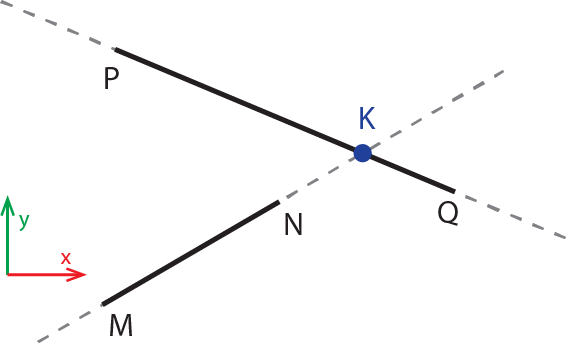
\includegraphics[scale=0.4]{Images/segments_intersection.png} 
    \caption{In this example segments do not collide because $max(M_x, N_x) = N_x \ngeq K_x$ or $max(M_y, N_y) \ngeq K_y$}
    \label{fig:segments:intersection}
\end{figure}

\subsection{Vertices ordering}
Given a set of unordered 2D points belonging to a convex hull, we want to sort them in a counterclockwise order, so that two consecutive vertices form an edge of the convex hull.

To do so we can compute the barycenter $O$ of the set of points that, being them part of a convex hull\footnote{We can state that the vertices we found so far make up a convex hull because the overlapping of two convex hulls is necessarily a convex hull.}, is necessarily inside the convex hull itself.

Now, for each vertex $A_k$ we can calculate the vector $\overrightarrow{OA_k}$, and sort the vertices based on $atan2(\overrightarrow{OA_k}_y, \overrightarrow{OA_K}_x)$.

The $atan2(v_y, v_x)$ function returns the angle between the positive x-axis and the vector $v=\langle v_x, v_y \rangle$. Differently from the arctangent function, the returned angle ranges in the interval $(-\pi, \pi]$, therefore is well suited for our purpose of sorting the convex hull vertices.

\begin{figure}[H]
    \centering
    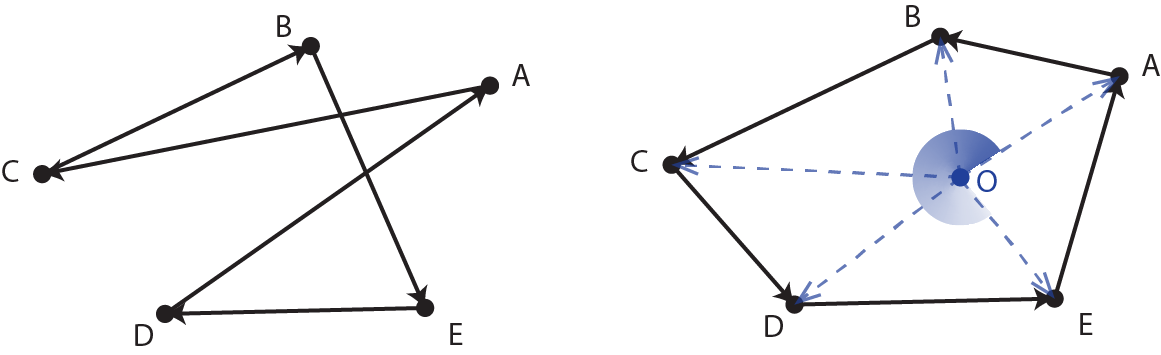
\includegraphics[scale=0.4]{Images/vertices_sorting.png} 
    \caption{Vertices of a convex hull before and after $atan2$ sorting.}
    \label{fig:vertices_sorting}
\end{figure}

\section{2D Hull Area Computation} \label{sec:2dHull_area_computation}
To calculate the area of a 2-dimensional hull we decided to use the Gauss's area formula, also known as the shoelace formula \cite{shoelace_formula}.

Given a polygon with vertices $P_0, P_1, ..., P_n$, where each vertex has coordinates: $P_k = (x_k, y_k)$, its area can be found with this formula:
\begin{align*}
	Area =& \bigg|\frac{1}{2}\cdot\left(\begin{vmatrix} x_0 & y_1\\y_0 & y_1 \end{vmatrix} + \begin{vmatrix} x_1 & y_2\\y_1 & y_2 \end{vmatrix} + ... + \begin{vmatrix} x_{n-1} & y_n\\y_{n-1} & y_n \end{vmatrix} + \begin{vmatrix} x_n & y_0\\y_n & y_0 \end{vmatrix}\right)\bigg|\\
	=& \Bigg|\frac{\displaystyle\sum_{i=0}^{n}(x_i \cdot y_{i+1} - y_i \cdot x_{i+1})}{2}\Bigg|
\end{align*}

In the last formula we consider $P_0 = P_{n+1}$.



% === Lists ===
\listoffigures
\listoftables

% Table of symbols
\chapter*{List of Symbols} % You have to include a chapter for your list of symbols (
\begin{table}[H]
    \centering
    \begin{tabular}{lll}
        \textbf{Symbol} & \textbf{Description} & \textbf{Unit} \\\hline\\[-9px]
        $\bm{alpha}$ & symbol 1 & km \\[2px]
    \end{tabular}
\end{table}

% === Ringraziamenti ===
\chapter*{Ringraziamenti}
\small
Lorem ipsum dolor sit amet, consectetur adipiscing elit, sed do eiusmod tempor incididunt ut labore et dolore magna aliqua. Ultricies integer quis auctor elit sed vulputate mi. Accumsan sit amet nulla facilisi morbi. Suspendisse potenti nullam ac tortor vitae purus faucibus. Ultricies lacus sed turpis tincidunt id. Sit amet mauris commodo quis imperdiet. Arcu bibendum at varius vel. Venenatis urna cursus eget nunc. Mus mauris vitae ultricies leo integer malesuada nunc vel. Sodales neque sodales ut etiam sit. Pellentesque dignissim enim sit amet venenatis urna cursus eget nunc. Condimentum mattis pellentesque id nibh tortor id aliquet lectus. Ultrices gravida dictum fusce ut placerat orci nulla pellentesque dignissim. Faucibus pulvinar elementum integer enim neque. Morbi tincidunt augue interdum velit euismod in pellentesque massa.

A diam maecenas sed enim ut sem viverra aliquet eget. Viverra aliquet eget sit amet tellus cras. Tellus at urna condimentum mattis pellentesque. Quis viverra nibh cras pulvinar. Posuere morbi leo urna molestie at elementum. Aenean euismod elementum nisi quis eleifend quam. In hac habitasse platea dictumst vestibulum rhoncus. Nullam non nisi est sit amet facilisis magna etiam tempor. Neque laoreet suspendisse interdum consectetur libero. Vitae auctor eu augue ut lectus arcu bibendum. Ipsum consequat nisl vel pretium lectus quam. Velit dignissim sodales ut eu sem. Odio morbi quis commodo odio. Lectus nulla at volutpat diam. Neque gravida in fermentum et sollicitudin ac. Nunc non blandit massa enim nec dui nunc. Quisque id diam vel quam elementum pulvinar etiam non quam. Consequat id porta nibh venenatis cras sed felis. Vitae justo eget magna fermentum iaculis eu non diam. Mi sit amet mauris commodo.
\normalsize

\ClearShipoutPicture

\triangleLogo
\end{document}
